%%
%% Automatically generated file from Doconce source
%% (https://github.com/hplgit/doconce/)
%%
% #ifdef PTEX2TEX_EXPLANATION
%%
%% The file follows the ptex2tex extended LaTeX format, see
%% ptex2tex: http://code.google.com/p/ptex2tex/
%%
%% Run
%%      ptex2tex myfile
%% or
%%      doconce ptex2tex myfile
%%
%% to turn myfile.p.tex into an ordinary LaTeX file myfile.tex.
%% (The ptex2tex program: http://code.google.com/p/ptex2tex)
%% Many preprocess options can be added to ptex2tex or doconce ptex2tex
%%
%%      ptex2tex -DMINTED -DPALATINO -DA6PAPER -DLATEX_HEADING=traditional myfile
%%      doconce ptex2tex myfile -DLATEX_HEADING=titlepage envir=minted
%%
%% ptex2tex will typeset code environments according to a global or local
%% .ptex2tex.cfg configure file. doconce ptex2tex will typeset code
%% according to options on the command line (just type doconce ptex2tex to
%% see examples). If doconce ptex2tex has envir=minted, it enables the
%% minted style without needing -DMINTED.
% #endif

% #ifndef LATEX_STYLE
% #define LATEX_STYLE "std"
% #endif

% #ifndef LATEX_HEADING
% #define LATEX_HEADING "doconce_heading"
% #endif

% #ifndef PREAMBLE
% #if LATEX_HEADING == "Springer_collection"
% #undef PREAMBLE
% #else
% #define PREAMBLE
% #endif
% #endif


% #ifdef PREAMBLE
%-------------------- begin preamble ----------------------
% #if LATEX_STYLE == "std"

\documentclass[%
twoside,                 % oneside: electronic viewing, twoside: printing
% #ifdef DOUBLE_SPACING
draft,                   % or final
% #else
final,                   % or draft (marks overfull hboxes)
% #endif
10pt]{article}

% #elif LATEX_STYLE == "Springer_lncse"
% Style: Lecture Notes in Computational Science and Engineering (Springer)
\documentclass[envcountsect,open=right]{lncse}
\pagestyle{headings}
% #elif LATEX_STYLE == "Springer_T2"
% Style: T2 (Springer)
\documentclass[graybox,sectrefs,envcountresetchap,open=right]{svmono}
\usepackage{t2}
\special{papersize=193mm,260mm}
% #elif LATEX_STYLE == "Springer_llcse"
% Style: Lecture Notes in Computer Science (Springer)
\documentclass[oribib]{llncs}
% #elif LATEX_STYLE == "Koma_Script"
% Style: Koma-Script
\documentclass[10pt]{scrartcl}
% #elif LATEX_STYLE == "siamltex"
% Style: SIAM LaTeX2e
\documentclass[leqno]{siamltex}
% #elif LATEX_STYLE == "siamltexmm"
% Style: SIAM LaTeX2e multimedia
\documentclass[leqno]{siamltexmm}
% #endif

\listfiles               % print all files needed to compile this document

% #ifdef A4PAPER
\usepackage[a4paper]{geometry}
% #endif
% #ifdef A6PAPER
% a6paper is suitable for mobile devices
\usepackage[%
  a6paper,
  text={90mm,130mm},
  inner={5mm},           % inner margin (two sided documents)
  top=5mm,
  headsep=4mm
  ]{geometry}
% #endif

\usepackage{relsize,epsfig,makeidx,color,setspace,amsmath,amsfonts}
\usepackage[table]{xcolor}
\usepackage{bm,microtype}

\usepackage{ptex2tex}

% #ifdef MINTED
\usepackage{minted}
\usemintedstyle{default}
% #endif

% #ifdef XELATEX
% xelatex settings
\usepackage{fontspec}
\usepackage{xunicode}
\defaultfontfeatures{Mapping=tex-text} % To support LaTeX quoting style
\defaultfontfeatures{Ligatures=TeX}
\setromanfont{Kinnari}
% Examples of font types (Ubuntu): Gentium Book Basic (Palatino-like),
% Liberation Sans (Helvetica-like), Norasi, Purisa (handwriting), UnDoum
% #else
\usepackage[T1]{fontenc}
%\usepackage[latin1]{inputenc}
\usepackage[utf8]{inputenc}
% #ifdef HELVETICA
% Set helvetica as the default font family:
\RequirePackage{helvet}
\renewcommand\familydefault{phv}
% #endif
% #ifdef PALATINO
% Set palatino as the default font family:
\usepackage[sc]{mathpazo}    % Palatino fonts
\linespread{1.05}            % Palatino needs extra line spread to look nice
% #endif
% #endif
\usepackage{lmodern}         % Latin Modern fonts derived from Computer Modern

% Hyperlinks in PDF:
\definecolor{linkcolor}{rgb}{0,0,0.4}
\usepackage[%
    colorlinks=true,
    linkcolor=linkcolor,
    urlcolor=linkcolor,
    citecolor=black,
    filecolor=black,
    %filecolor=blue,
    pdfmenubar=true,
    pdftoolbar=true,
    bookmarksdepth=3   % Uncomment (and tweak) for PDF bookmarks with more levels than the TOC
            ]{hyperref}
%\hyperbaseurl{}   % hyperlinks are relative to this root

\setcounter{tocdepth}{2}  % number chapter, section, subsection

% Tricks for having figures close to where they are defined:
% 1. define less restrictive rules for where to put figures
\setcounter{topnumber}{2}
\setcounter{bottomnumber}{2}
\setcounter{totalnumber}{4}
\renewcommand{\topfraction}{0.85}
\renewcommand{\bottomfraction}{0.85}
\renewcommand{\textfraction}{0.15}
\renewcommand{\floatpagefraction}{0.7}
% 2. ensure all figures are flushed before next section
\usepackage[section]{placeins}
% 3. enable begin{figure}[H] (often leads to ugly pagebreaks)
%\usepackage{float}\restylefloat{figure}

\usepackage[framemethod=TikZ]{mdframed}

% --- begin definitions of admonition environments ---

% Admonition is an oval gray box
\newmdenv[
  backgroundcolor=gray!5,  %% white with 5%% gray
  skipabove=\topsep,
  skipbelow=\topsep,
  outerlinewidth=0,
  leftmargin=0,
  rightmargin=0,
  roundcorner=5,
  needspace=0pt,
]{graybox1mdframed}

\newenvironment{graybox1admon}[1][]{
\begin{graybox1mdframed}[frametitle=#1]
}
{
\end{graybox1mdframed}
}

% --- end of definitions of admonition environments ---

% prevent orhpans and widows
\clubpenalty = 10000
\widowpenalty = 10000

% #ifndef SECTION_HEADINGS
% #define SECTION_HEADINGS "std"
% #else
% http://www.ctex.org/documents/packages/layout/titlesec.pdf
\usepackage[compact]{titlesec}  % reduce the spacing above/below the heading
% #endif
% #if SECTION_HEADINGS == "blue"
% --- section/subsection headings with blue color ---
\definecolor{seccolor}{cmyk}{.9,.5,0,.35}  % siamltexmm.sty section color
\titleformat{name=\section}
{\color{seccolor}\normalfont\Large\bfseries}
{\color{seccolor}\thesection}{1em}{}
\titleformat{name=\subsection}
{\color{seccolor}\normalfont\large\bfseries}
{\color{seccolor}\thesubsection}{1em}{}
\titleformat{name=\paragraph}[runin]
{\color{seccolor}\normalfont\normalsize\bfseries}
{}{}{\indent}
% #ifdef FANCY_HEADER
% let the header have a thick gray hrule with section and page in blue above
\renewcommand{\headrulewidth}{0.4pt}
\renewcommand{\headrule}{{\color{gray!50}%
\hrule width\headwidth height\headrulewidth \vskip-\headrulewidth}}
\fancyhead[LE,RO]{{\color{seccolor}\rightmark}} %section
\fancyhead[RE,LO]{{\color{seccolor}\thepage}}
% #endif
% #elif SECTION_HEADINGS == "strongblue"
% --- section/subsection headings with a strong blue color ---
\definecolor{seccolor}{rgb}{0.2,0.2,0.8}
\titleformat{name=\section}
{\color{seccolor}\normalfont\Large\bfseries}
{\color{seccolor}\thesection}{1em}{}
\titleformat{name=\subsection}
{\color{seccolor}\normalfont\large\bfseries}
{\color{seccolor}\thesubsection}{1em}{}
\titleformat{name=\paragraph}[runin]
{\color{seccolor}\normalfont\normalsize\bfseries}
{}{}{\indent}
% #elif SECTION_HEADINGS == "gray"
% --- section/subsection headings with white text on gray background ---
\titleformat{name=\section}[block]
  {\sffamily\Large}{}{0pt}{\colorsection}
\titlespacing*{\section}{0pt}{\baselineskip}{\baselineskip}

\newcommand{\colorsection}[1]{%
  \colorbox{gray!50}{{\color{white}\thesection\ #1}}}

\titleformat{name=\subsection}[block]
  {\sffamily\large}{}{0pt}{\colorsubsection}
\titlespacing*{\subsection}{0pt}{\baselineskip}{\baselineskip}

\newcommand{\colorsubsection}[1]{%
  \colorbox{gray!50}{{\color{white}\thesubsection\ #1}}}
% #elif SECTION_HEADINGS == "gray-wide"
% --- section/subsection headings with white text on wide gray background ---
\titleformat{name=\section}[block]
  {\sffamily\Large}{}{0pt}{\colorsection}
\titlespacing*{\section}{0pt}{\baselineskip}{\baselineskip}

\newcommand{\colorsection}[1]{%
  \colorbox{gray!50}{\parbox{\dimexpr\textwidth-2\fboxsep}%
           {\color{white}\thesection\ #1}}}

\titleformat{name=\subsection}[block]
  {\sffamily\large}{}{0pt}{\colorsubsection}
\titlespacing*{\subsection}{0pt}{\baselineskip}{\baselineskip}

\newcommand{\colorsubsection}[1]{%
  \colorbox{gray!50}{\parbox{\dimexpr\textwidth-2\fboxsep}%
           {\color{white}\thesubsection\ #1}}}
% #endif

% #ifdef COLORED_TABLE_ROWS
% color every two table rows
\let\oldtabular\tabular
\let\endoldtabular\endtabular
% #if COLORED_TABLE_ROWS not in ("gray", "blue")
% #define COLORED_TABLE_ROWS gray
% #endif
% #else
% #define COLORED_TABLE_ROWS no
% #endif
% #if COLORED_TABLE_ROWS == "gray"
\definecolor{rowgray}{gray}{0.9}
\renewenvironment{tabular}{\rowcolors{2}{white}{rowgray}%
\oldtabular}{\endoldtabular}
% #elif COLORED_TABLE_ROWS == "blue"
\definecolor{appleblue}{rgb}{0.93,0.95,1.0}  % Apple blue
\renewenvironment{tabular}{\rowcolors{2}{white}{appleblue}%
\oldtabular}{\endoldtabular}
% #endif


% --- end of standard preamble for documents ---


% insert custom LaTeX commands...

\raggedbottom
\makeindex

%-------------------- end preamble ----------------------

\begin{document}

% #endif


% ------------------- main content ----------------------



% ----------------- title -------------------------

% #if LATEX_HEADING == "traditional"

% #if SECTION_HEADINGS in ("blue", "strongblue")
\title{{\color{seccolor} On Schemes for Exponential Decay}}
% #else
\title{On Schemes for Exponential Decay}
% #endif

% #elif LATEX_HEADING == "titlepage"

\thispagestyle{empty}
\hbox{\ \ }
\vfill
\begin{center}
{\huge{\bfseries{
\begin{spacing}{1.25}
% #if SECTION_HEADINGS in ("blue", "strongblue")
{\color{seccolor}\rule{\linewidth}{0.5mm}} \\[0.4cm]
{\color{seccolor}On Schemes for Exponential Decay}
\\[0.4cm] {\color{seccolor}\rule{\linewidth}{0.5mm}} \\[1.5cm]
% #else
{\rule{\linewidth}{0.5mm}} \\[0.4cm]
{On Schemes for Exponential Decay}
\\[0.4cm] {\rule{\linewidth}{0.5mm}} \\[1.5cm]
% #endif
\end{spacing}
}}}

% #elif LATEX_HEADING == "Springer_collection"
\title*{On Schemes for Exponential Decay}
% Short version of title:
\titlerunning{On Schemes for Exponential Decay}

% #elif LATEX_HEADING == "beamer"
\title{On Schemes for Exponential Decay}
% #else
\thispagestyle{empty}

\begin{center}
{\LARGE\bf
\begin{spacing}{1.25}
On Schemes for Exponential Decay
\end{spacing}
}
\end{center}
% #endif

% ----------------- author(s) -------------------------
% #if LATEX_HEADING == "traditional"
\author{Hans Petter Langtangen\footnote{Center for Biomedical Computing, Simula Research Laboratory and Department of Informatics, University of Oslo.}}

% #elif LATEX_HEADING == "titlepage"
\vspace{1.3cm}

    {\Large\textsf{Hans Petter Langtangen${}^{1, 2}$}}\\ [3mm]
    
\ \\ [2mm]

{\large\textsf{${}^1$Center for Biomedical Computing, Simula Research Laboratory} \\ [1.5mm]}
{\large\textsf{${}^2$Department of Informatics, University of Oslo} \\ [1.5mm]}
% #elif LATEX_HEADING == "Springer_collection"

\author{Hans Petter Langtangen}
% Short version of authors:
%\authorrunning{...}
\institute{Hans Petter Langtangen\at Center for Biomedical Computing, Simula Research Laboratory and Department of Informatics, University of Oslo}

% #elif LATEX_HEADING == "beamer"
\author{Hans Petter Langtangen\inst{1,2}}
\institute{Center for Biomedical Computing, Simula Research Laboratory\inst{1}
\and
Department of Informatics, University of Oslo\inst{2}}
% #else

\begin{center}
{\bf Hans Petter Langtangen${}^{1, 2}$} \\ [0mm]
\end{center}

\begin{center}
% List of all institutions:
\centerline{{\small ${}^1$Center for Biomedical Computing, Simula Research Laboratory}}
\centerline{{\small ${}^2$Department of Informatics, University of Oslo}}
\end{center}
% #endif
% ----------------- end author(s) -------------------------


% #if LATEX_HEADING == "traditional"
\date{Jan 8, 2014}
\maketitle
% #elif LATEX_HEADING == "beamer"
\date{Jan 8, 2014
% <titlepage figure>
}
% #elif LATEX_HEADING == "titlepage"

\ \\ [10mm]
{\large\textsf{Jan 8, 2014}}

\end{center}
\vfill
\clearpage

% #else
\begin{center}
Jan 8, 2014
\end{center}

\vspace{1cm}

% #endif


\begin{center}  % inline figure
  \centerline{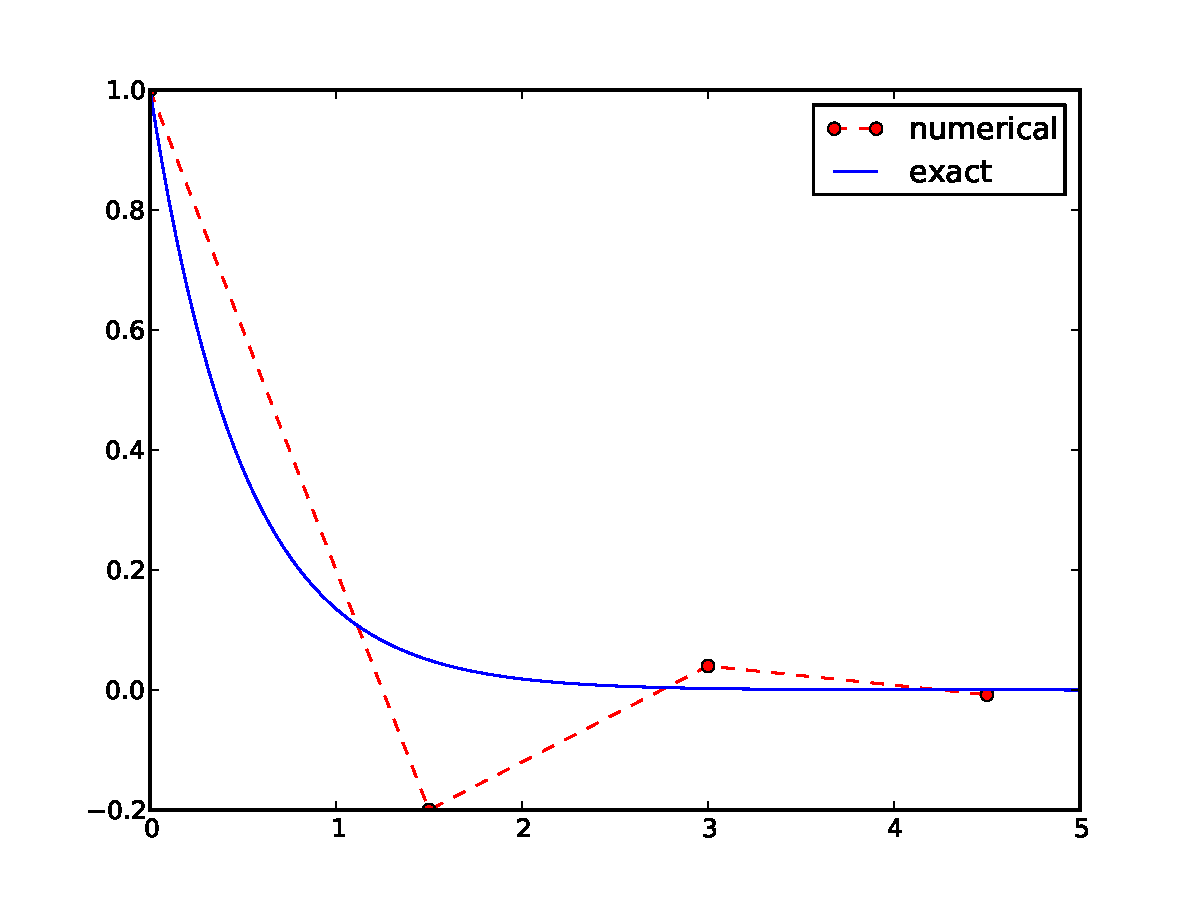
\includegraphics[width=0.4\linewidth]{fig/CN_logo.pdf}}
\end{center}



% !split

\section{Goal}

The primary goal of this demo talk is to demonstrate how to write
talks with \href{{https://github.com/hplgit/doconce}}{Doconce}
and get them rendered in numerous HTML formats.

\begin{graybox1admon}[Layout.]
This version
utilizes latex document slides with the theme \code{no theme}.
\end{graybox1admon}






% !bnotes
The talk investigates the accuracy of three finite difference
schemes for the ordinary differential equation $u'=-au$ with the
aid of numerical experiments. Numerical artifacts are in particular
demonstrated.
% !enotes


% !split
\section{Mathematical problem}


% !bslidecell 00


\begin{align}
u'(t) &= -au(t),
\label{ode}\\ 
u(0)  &= I,
\label{initial:value}
\end{align}

\begin{itemize}
 \item $t\in (0,T]$

 \item $a$, $I$, and $T$ are prescribed parameters

 \item $u(t)$ is the unknown function
\end{itemize}

\noindent
% !eslidecell


% !bslidecell 01

\begin{center}  % inline figure
  \centerline{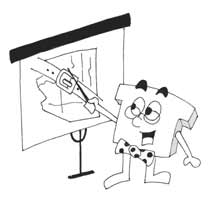
\includegraphics[width=0.5\linewidth]{fig/teacher2.jpg}}
\end{center}

% !eslidecell

% !split
\section{Numerical solution method}


% !bpop
\begin{itemize}
 \item Mesh in time: $0= t_0< t_1 \cdots < t_N=T$

 \item Assume constant $\Delta t = t_{n}-t_{n-1}$

 \item $u^n$: numerical approx to the exact solution at $t_n$
\end{itemize}

\noindent
% !epop

% !bpop
Numerical scheme:
   \[
   u^{n+1} = \frac{1 - (1-\theta) a\Delta t}{1 + \theta a\Delta t}u^n,
   \quad n=0,1,\ldots,N-1
   \]
% !epop


% !split

\section{Implementation}

The numerical method is implemented in a Python function:

\bpycod
def solver(I, a, T, dt, theta):
    """Solve u'=-a*u, u(0)=I, for t in (0,T] with steps of dt."""
    dt = float(dt)           # avoid integer division
    N = int(round(T/dt))     # no of time intervals
    T = N*dt                 # adjust T to fit time step dt
    u = zeros(N+1)           # array of u[n] values
    t = linspace(0, T, N+1)  # time mesh

    u[0] = I                 # assign initial condition
    for n in range(0, N):    # n=0,1,...,N-1
        u[n+1] = (1 - (1-theta)*a*dt)/(1 + theta*dt*a)*u[n]
    return u, t
\epycod

% !split
\subsection{The Crank-Nicolson method}



\begin{center}  % inline figure
  \centerline{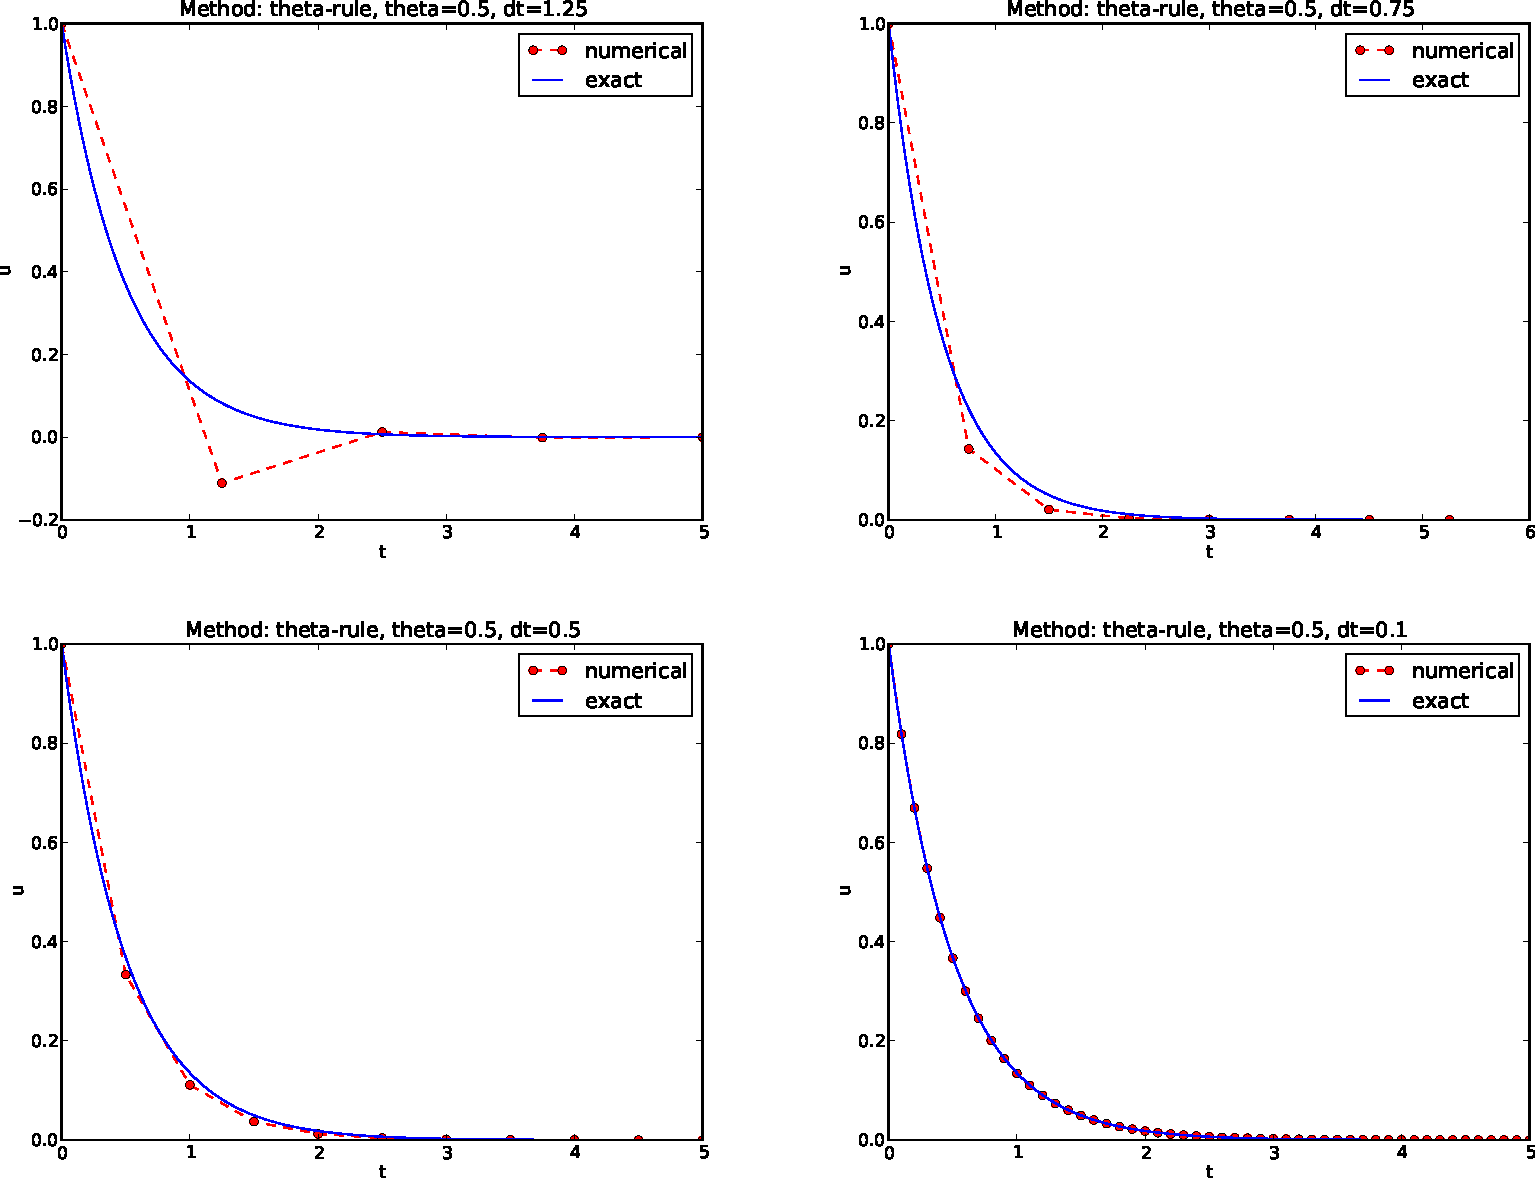
\includegraphics[width=0.9\linewidth]{fig/CN.pdf}}
\end{center}


% !split
\subsection{The artifacts can be explained by some theory}

% !bpop
Exact solution of the scheme:

\[ u^n = A^n,\quad A = \frac{1 - (1-\theta) a\Delta t}{1 + \theta a\Delta t}\thinspace .\]
% !epop

% !bpop
\begin{itemize}
 \item Stability: $|A| < 1$

 \item No oscillations: $A>0$

 \item Always for Backward Euler ($\theta=1$)

 \item $\Delta t < 1/a$ for Forward Euler ($\theta=0$)

 \item $\Delta t < 2/a$ for Crank-Nicolson ($\theta=1/2$)
\end{itemize}

\noindent
% !epop

% !bpop

\begin{graybox1admon}[Concluding remarks:]
Only the Backward Euler scheme is guaranteed to always give
qualitatively correct results.
\end{graybox1admon}


% !epop

% ------------------- end of main content ---------------


% #ifdef PREAMBLE
\printindex

\end{document}
% #endif

